% Krydo — Professional pitch deck (Beamer)
% Compile:
%   cd docs
%   pdflatex krydo-stellar-presentation.tex
%   pdflatex krydo-stellar-presentation.tex
% Output: krydo-stellar-presentation.pdf

\documentclass[aspectratio=169,11pt]{beamer}

% ── Theme & colours (aligned with docs/krydo-stellar-business-plan.tex) ─────
\usetheme{Madrid}
\usecolortheme{default}

\definecolor{StellarBlue}{HTML}{14B6E7}
\definecolor{StellarDark}{HTML}{0B3D4C}
\definecolor{AccentGold}{HTML}{C9A227}
\definecolor{BodyGray}{HTML}{374151}
\definecolor{LightBg}{HTML}{F3F7FA}

\setbeamercolor{palette primary}{bg=StellarDark, fg=white}
\setbeamercolor{palette secondary}{bg=StellarBlue, fg=white}
\setbeamercolor{palette tertiary}{bg=StellarDark!85, fg=white}
\setbeamercolor{structure}{fg=StellarBlue}
\setbeamercolor{title}{fg=white}
\setbeamercolor{frametitle}{bg=StellarDark, fg=white}
\setbeamercolor{block title}{bg=StellarDark, fg=white}
\setbeamercolor{block body}{bg=LightBg, fg=BodyGray}
\setbeamercolor{alerted text}{fg=AccentGold}

\setbeamertemplate{navigation symbols}{}
\setbeamertemplate{footline}{
  \leavevmode%
  \hbox{%
    \begin{beamercolorbox}[wd=.5\paperwidth,ht=2.6ex,dp=1.2ex,leftskip=1em]{author in head/foot}%
      \usebeamerfont{author in head/foot}\insertshortauthor
    \end{beamercolorbox}%
    \begin{beamercolorbox}[wd=.5\paperwidth,ht=2.6ex,dp=1.2ex,rightskip=1em]{date in head/foot}%
      \usebeamerfont{date in head/foot}\insertshortdate\hspace*{1.5em}\insertframenumber{} / \inserttotalframenumber
    \end{beamercolorbox}%
  }%
  \vskip0pt%
}

\usepackage[utf8]{inputenc}
\usepackage[T1]{fontenc}
\usepackage{lmodern}
\usepackage{microtype}
\usepackage{booktabs}
\usepackage{tabularx}
\usepackage{array}
\usepackage{tikz}
\usetikzlibrary{arrows.meta, positioning, shapes.geometric}
\usepackage[hidelinks]{hyperref}
\usepackage{url}

\newcommand{\krydo}{\textbf{Krydo}}
\newcommand{\mono}[1]{\texttt{\small #1}}

\title{Krydo}
\subtitle{Privacy-Preserving Financial Trust on Stellar}
\author{Nishant Agarwal}
\institute{Stellar Testnet \textbar\ Soroban Smart Contracts}
\date{July 2026}

\begin{document}

% ── Title ───────────────────────────────────────────────────────────────────
\begin{frame}[plain]
  \begin{tikzpicture}[remember picture, overlay]
    \fill[StellarDark] (current page.north west) rectangle (current page.south east);
    \fill[StellarBlue] ([yshift=0cm]current page.south west) rectangle ([yshift=0.35cm]current page.south east);
    \node[anchor=center, text=white, align=center] at (current page.center) {
      \begin{minipage}{0.88\paperwidth}
        {\fontsize{36}{40}\selectfont\bfseries Krydo}\\[0.4em]
        {\fontsize{16}{20}\selectfont Prove you qualify --- without revealing what you have}\\[1.8em]
        {\fontsize{12}{14}\selectfont\color{white!85}
          Verifiable credentials \textbullet\ Zero-knowledge proofs \textbullet\ Stellar Soroban}\\[2.2em]
        {\fontsize{11}{13}\selectfont\color{AccentGold!90!white}
          Live demo: \url{https://krydo-stellar.vercel.app}}\\[0.3em]
        {\fontsize{10}{12}\selectfont\color{white!70}
          GitHub: \url{https://github.com/nishant-uxs/krydo-stellar}}
      \end{minipage}
    };
  \end{tikzpicture}
\end{frame}

% ── Problem ─────────────────────────────────────────────────────────────────
\begin{frame}{The Problem}
  \begin{block}{Verification today over-collects}
    A lender asking \emph{``Do you earn at least INR\,10\,L?''} often receives:
  \end{block}
  \vspace{0.4em}
  \begin{columns}[T]
    \column{0.48\textwidth}
    \begin{itemize}
      \item Exact salary \& employer
      \item Bank statements
      \item PAN / national ID copies
    \end{itemize}
    \column{0.48\textwidth}
    \begin{itemize}
      \item Data cannot be revoked once leaked
      \item Re-sold across brokers
      \item High compliance \& breach risk
    \end{itemize}
  \end{columns}
  \vspace{0.6em}
  \begin{alertblock}{What we need}
    Prove a \textbf{predicate} (\texttt{score $\geq$ 700}, \texttt{income $\geq$ 10L}) --- not the underlying value.
  \end{alertblock}
\end{frame}

% ── Solution ────────────────────────────────────────────────────────────────
\begin{frame}{Our Solution}
  \krydo{} is a three-tier trust network on \textbf{Stellar Soroban}:
  \vspace{0.5em}
  \begin{center}
    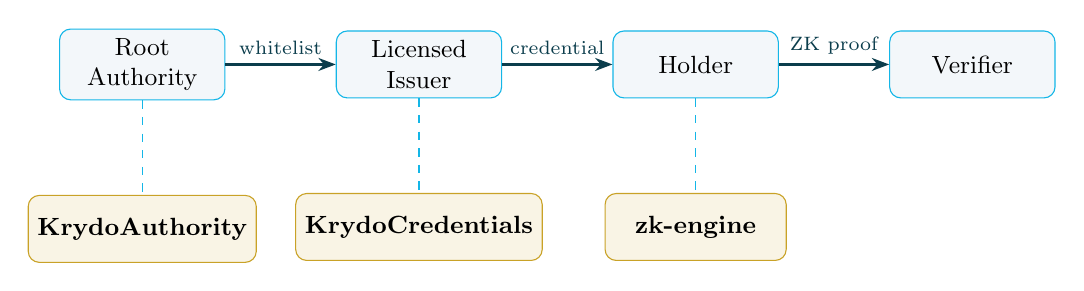
\begin{tikzpicture}[
      node distance=1.1cm and 1.4cm,
      actor/.style={draw=StellarBlue, fill=LightBg, rounded corners=4pt,
        minimum width=2.1cm, minimum height=0.85cm, align=center, font=\small},
      contract/.style={draw=AccentGold, fill=AccentGold!12, rounded corners=4pt,
        minimum width=2.3cm, minimum height=0.85cm, align=center, font=\small\bfseries},
      arr/.style={-{Stealth[length=2.2mm]}, thick, StellarDark}
    ]
      \node[actor] (root) {Root\\Authority};
      \node[actor, right=of root] (iss) {Licensed\\Issuer};
      \node[actor, right=of iss] (usr) {Holder};
      \node[actor, right=of usr] (ver) {Verifier};
      \draw[arr] (root) -- node[above, font=\scriptsize]{whitelist} (iss);
      \draw[arr] (iss) -- node[above, font=\scriptsize]{credential} (usr);
      \draw[arr] (usr) -- node[above, font=\scriptsize]{ZK proof} (ver);
      \node[contract, below=1.2cm of iss] (kc) {KrydoCredentials};
      \node[contract, below=1.2cm of root] (ka) {KrydoAuthority};
      \node[contract, below=1.2cm of usr] (zk) {zk-engine};
      \draw[dashed, StellarBlue] (iss) -- (kc);
      \draw[dashed, StellarBlue] (root) -- (ka);
      \draw[dashed, StellarBlue] (usr) -- (zk);
    \end{tikzpicture}
  \end{center}
\end{frame}

% ── How it works ────────────────────────────────────────────────────────────
\begin{frame}{End-to-End Flow}
  \small
  \begin{enumerate}
    \item \textbf{Issuer} (whitelisted on-chain) signs \texttt{issue\_credential} $\rightarrow$ hash on ledger, plaintext off-chain
    \item \textbf{Holder} generates a \textbf{sigma-protocol ZK proof} in the browser (Pedersen + Fiat--Shamir)
    \item \textbf{Verifier} calls \texttt{POST /api/zk/verify} --- learns only whether the predicate holds
    \item Optional: holder wallet-signs \texttt{KrydoAudit.anchor} for a public audit trail
  \end{enumerate}
  \vspace{0.5em}
  \begin{block}{Design principle}
    Blockchain = source of truth for \emph{what exists}. Firestore = fast query layer. Private keys never leave the wallet.
  \end{block}
\end{frame}

% ── ZK ──────────────────────────────────────────────────────────────────────
\begin{frame}{Zero-Knowledge Layer}
  \begin{columns}[T]
    \column{0.52\textwidth}
    \textbf{Not SNARKs --- real sigma protocols}
    \begin{itemize}
      \item Pedersen commitments $C = vG + rH$
      \item Fiat--Shamir non-interactivity
      \item No trusted setup, no circuits
      \item Proofs in milliseconds (browser + API)
    \end{itemize}
    \vspace{0.4em}
  \textbf{Proof types:}
    \texttt{range\_above}, \texttt{range\_below}, \texttt{equality}, \texttt{membership}, \texttt{selective\_disclosure}
    \column{0.45\textwidth}
    \begin{block}{Example}
      Credential: credit score \textbf{782}\\[0.3em]
      Proof shared: \textbf{score $\geq$ 750}\\[0.3em]
      Verifier learns: predicate is \textbf{true}\\[0.3em]
      Verifier does \textbf{not} learn: 782
    \end{block}
  \end{columns}
\end{frame}

% ── Smart contracts ─────────────────────────────────────────────────────────
\begin{frame}{Soroban Smart Contracts}
  \begin{table}
    \small
    \renewcommand{\arraystretch}{1.35}
    \begin{tabularx}{\textwidth}{@{}l X@{}}
      \toprule
      \textbf{Contract} & \textbf{Responsibility} \\
      \midrule
      \texttt{KrydoAuthority} & Root-controlled issuer whitelist (\texttt{add\_issuer}, \texttt{revoke\_issuer}) \\
      \texttt{KrydoCredentials} & Credential hashes, issuance, revocation on-chain \\
      \texttt{KrydoAudit} & Stateless event log for wallet-signed anchors (requests, roles, ZK) \\
      \bottomrule
    \end{tabularx}
  \end{table}
  \vspace{0.3em}
  \begin{itemize}
    \item Auth: \textbf{Sign-in-with-Stellar} (SEP-53) $\rightarrow$ JWT
    \item Every state-changing tx: in-app confirm $\rightarrow$ \textbf{wallet signature}
    \item Wallets: Freighter, xBull, Lobstr, Hana via Stellar Wallets Kit
  \end{itemize}
\end{frame}

% ── Testnet addresses ───────────────────────────────────────────────────────
\begin{frame}[fragile]{Deployed on Stellar Testnet}
  \small
  \textbf{Network:} Testnet \quad
  \textbf{Deployed:} 11 July 2026 \quad
  \textbf{Explorer:} \url{https://stellar.expert/explorer/testnet}
  \vspace{0.5em}

  \begin{table}
    \renewcommand{\arraystretch}{1.4}
    \begin{tabularx}{\textwidth}{@{}l >{\raggedright\arraybackslash}X@{}}
      \toprule
      \textbf{Role / Contract} & \textbf{Address (StrKey)} \\
      \midrule
      Root authority & \mono{GC5VBHY5DWV7NTL4PCQL3XGOE4FY2DJHM2JYLRC6YS2IHYTPDZ4DOFIU} \\
      KrydoAuthority & \mono{CDBYAPYW34OCTNMTT3H75XLC2JRA7HD4ULA5YVJ75SISM67GPCD6FNK2} \\
      KrydoCredentials & \mono{CD7PFDNVL2V4SO4WQWP225CJRYV24GIGM3ZALS2WHIEM6UINQK7KJCOV} \\
      KrydoAudit & \mono{CALAZRCMK2POSKYEXA7LB3SPIBU5555SD5LX53LHC2YYCSZMYEQVXJSX} \\
      \bottomrule
    \end{tabularx}
  \end{table}
  \vspace{0.2em}
  \footnotesize
  RPC: \mono{https://soroban-testnet.stellar.org}
\end{frame}

% ── Tech stack ────────────────────────────────────────────────────────────────
\begin{frame}{Technology Stack}
  \begin{columns}[T]
    \column{0.48\textwidth}
    \textbf{On-chain}
    \begin{itemize}
      \item Soroban (Rust / WASM)
      \item Stellar Testnet
      \item Sub-cent tx fees
    \end{itemize}
    \textbf{Backend}
    \begin{itemize}
      \item Node.js + Express
      \item Firestore (mirror + queries)
      \item Zod validation, JWT auth
    \end{itemize}
    \column{0.48\textwidth}
    \textbf{Frontend}
    \begin{itemize}
      \item React + Vite + TypeScript
      \item Stellar Wallets Kit
      \item Client-side ZK engine
    \end{itemize}
    \textbf{Quality}
    \begin{itemize}
      \item 168 unit tests, CI on GitHub Actions
      \item Open source (MIT)
    \end{itemize}
  \end{columns}
\end{frame}

% ── Security ────────────────────────────────────────────────────────────────
\begin{frame}{Security \& Trust Model}
  \begin{columns}[T]
    \column{0.55\textwidth}
    \begin{itemize}
      \item Four roles: Root, Issuer, Holder, Verifier
      \item No role can elevate itself
      \item On-chain \texttt{require\_auth} for issuance
      \item Claim summary vs.\ value consistency checks
      \item Issuer list synced from \texttt{KrydoAuthority}
    \end{itemize}
    \column{0.42\textwidth}
    \begin{alertblock}{MVP status}
      Testnet deployment. External crypto audit and multi-sig root recommended before production finance use.
    \end{alertblock}
  \end{columns}
\end{frame}

% ── Roadmap ─────────────────────────────────────────────────────────────────
\begin{frame}{Roadmap}
  \begin{table}
    \small
    \renewcommand{\arraystretch}{1.3}
    \begin{tabularx}{\textwidth}{@{}l X@{}}
      \toprule
      \textbf{Phase} & \textbf{Milestone} \\
      \midrule
      Done & Testnet contracts, multi-wallet SIWS, wallet-signed txs, live demo \\
      Next & Mainnet deploy ($\sim$100--102 XLM operating budget), demo issuers, waitlist \\
      Future & Multi-sig root, encrypted credential store (IPFS/Arweave), mainnet partners \\
      \bottomrule
    \end{tabularx}
  \end{table}
  \vspace{0.4em}
  \begin{block}{Mainnet operating budget (approx.)}
    \textbf{100--102 XLM} total --- contract deploy \& integration testing $\sim$2--5 XLM;
    balance held as reserve for demo issuers, storage rent (TTL), and 12-month on-chain operations.
  \end{block}
  \vspace{0.3em}
  \begin{block}{Try it now}
    \url{https://krydo-stellar.vercel.app} \quad Connect wallet on \textbf{Testnet}
  \end{block}
\end{frame}

% ── Thank you ───────────────────────────────────────────────────────────────
\begin{frame}[plain]
  \begin{tikzpicture}[remember picture, overlay]
    \fill[StellarDark] (current page.north west) rectangle (current page.south east);
    \node[anchor=center, text=white, align=center] at (current page.center) {
      \begin{minipage}{0.85\paperwidth}
        {\fontsize{32}{36}\selectfont\bfseries Thank you}\\[1.2em]
        {\fontsize{14}{18}\selectfont Questions?}\\[1.8em]
        {\fontsize{11}{14}\selectfont
          Demo: \url{https://krydo-stellar.vercel.app}\\[0.4em]
          Repo: \url{https://github.com/nishant-uxs/krydo-stellar}\\[0.4em]
          Docs: \texttt{DOCUMENTATION.md}
        }
      \end{minipage}
    };
  \end{tikzpicture}
\end{frame}

\end{document}
